\chapter{Event Categorisation}
\label{chap:categorisation}

\section{Introduction}

The event selection consists of the preselection described in Chapter~\ref{chap:objects}, 
and in addition requires the two leading preselected photon candidates to have 
$\pt^{\gamma 1} > \mgg/3$ and $\pt^{\gamma 2} > \mgg /4$ respectively, 
with an invariant mass in the range $100 < \mgg < \SI{180}{GeV}$.
Both photons must also satisfy the
pseudo-rapidity requirement $|\eta|<2.5$ and must not be in the barrel-endcap
transition region $1.44 < |\eta| < 1.57$.
The above $\eta$ requirement is applied to the photo supercluster
position, and the requirement on the photon $\pt$ is applied 
after the vertex assignment.

The \Hgg analysis depends on the ability to distinguish the narrow signal peak 
from the smoothly falling background in the diphoton mass distribution.
Selected events are therefore subject to further categorisation, in order to 
increase the ratio of the number of signal events to the number of background events (S/B).
This enhances the sensitivity of the analysis, 
reducing the expected uncertainties on the measured quantities.

Analysis categories are also constructed to target events in which the Higgs boson was 
produced by a specific production mechanism. 
This is achieved using the information provided by additional objects in the event, 
alongside the two photons arising from the Higgs boson decay.
As well as facilitating measurements of cross sections corresponding 
to individual production mechanisms, these dedicated categories also enable the S/B to be improved.

In the previous \Hgg analysis using the 2016 dataset \cite{HIG-16-040}, 
dedicated categories targeting the VBF, ttH, and VH modes were constructed, 
with the remaining so-called ``Untagged" categories composed mostly of ggH events.
Here a similar approach is employed, 
but with additional divisions targeting individual stage 1 bins for the ggH and VBF processes.
Events selected by the 2017 \Hgg analysis targeting ttH production, 
described in Ref.~\cite{HIG-18-018}, are not included in this analysis. 
This is achieved by first applying the same selection criteria used to construct the ttH categories, 
and then removing them from further consideration. 
There are no dedicated analysis categories for VH production.

The categorisation targeting ggH is based on the reconstructed diphoton transverse momentum (\ptgg) 
and the number of jets in the event. 
A BDT referred to as the diphoton BDT is then used to reduce the amount of background. 
The VBF analysis categories make use of the same diphoton BDT 
to reduce the number of background events. 
Additionally, a BDT targeting the kinematics of the characteristic VBF dijet system, 
known as the dijet BDT, is utilised to reduce the contamination from ggH events.

Due to the conditions differing between the two years, 
the analysis is optimised separately for the 2016 and 2017 datasets. 
A simultaneous fit to the categories from both years is then performed to estimate the 
values of the parameters of interest and their uncertainties (described in Chapter ~\ref{chap:results}).
The remainder of this chapter describes in detail the training of the diphoton and dijet BDTs, 
and their use in the category optimisation process for both ggH and VBF events

\section{Gluon fusion categorisation}
\subsection{Signal bin definitions}

At stage 1 of the STXS framework, 
the gluon fusion process (ggH) is divided into a total of eleven particle level bins.
The events are split first by the number of jets, 
defined at particle level using the anti-$k_T$ algorithm with radius parameter 0.4 
and jet $\pt > \SI{30}{GeV}$~\cite{AntiKt}.
All stable particles except for the decay products of the Higgs boson 
are included in the anti-$k_T$ clustering.
There are zero (0J), one (1J), and greater than or equal to two (2J) jets bins.
In events with at least one jet, a further splitting 
by the value of the transverse momentum of the Higgs boson (\ptH) is performed. 
Four bins are defined by boundaries placed at 60, 120, and \SI{200}{GeV}.
These bins are denoted as low, medium (med), high, and BSM, respectively.
Finally, a separate ggH region is dedicated to the vector boson fusion-like phase space, 
for which a pair of jets (a dijet) with invariant mass $m_{jj} > \SI{400}{GeV}$ 
and difference in pseudorapidity $\Delta\eta > 2.8$ is required.
The dijet is formed from the two leading jets in the event.
This region is split into two-jet-like ($\ptHjj < \SI{25}{GeV}$) 
and three-jet-like ($\ptHjj > \SI{25}{GeV}$) bins, 
where \ptHjj is defined as the transverse momentum of the Higgs boson plus dijet system.
Each bin is exclusive; events included in the VBF-like region are not included in the other ggH 2J bins.
A table summarising the definition of each bin, its cross section, and the fraction of the 
total ggH cross section is shown in Table \ref{tab:cat_ggHfractions}.
The inclusive ggH cross section is $48.52~\textrm{pb}$ at $\mH = \SI{125.09}{GeV}$, 
computed to an accuracy of three loops in perturbative quantum chromodynamics (QCD) 
and next-to-leading order (NLO) in electroweak perturbations (EW) 
\cite{YR4,Anastasiou2015,Anastasiou2016}.
Of this approximately $44.2~\textrm{pb}$ is within $|y_H| < 2.5$.

\begin{table}
  \begin{centering}
    \begin{tabular}{ r | c | c | c } 
    \hline
    Region & Definition & Fraction & Cross section (pb) \\ 
    \hline
    0J          & Exactly zero jets, any $\ptH$               & 60.0\% & 26.49 \\ 
    \hline
    1J low      & Exactly one jet, $\ptH <$ 60 GeV            & 15.4\% & 6.79  \\
    \hline
    1J med      & Exactly one jet, 60 GeV $< \ptH <$ 120 GeV  & 10.4\% & 4.61  \\ 
    \hline
    1J high     & Exactly one jet, 120 GeV $< \ptH <$ 200 GeV & 1.7\% & 0.76   \\
    \hline
    1J BSM      & Exactly one jet, $\ptH >$ 200 GeV           & 0.4\% & 0.16   \\ 
    \hline
    2J low      & $\ge$ two jets, $\ptH <$ 60 GeV             & 2.9\% & 1.26   \\
    \hline
    2J med      & $\ge$ two jets, 60 GeV $< \ptH <$ 120 GeV   & 4.5\% & 2.00   \\ 
    \hline
    2J high     & $\ge$ two jets, 120 GeV $< \ptH <$ 200 GeV  & 2.3\% & 1.00   \\
    \hline
    2J BSM      & $\ge$ two jets, $\ptH >$ 200 GeV            & 1.0\% & 0.43   \\ 
    \hline
    \multirow{2}{*}{VBF-like 2J} & $\ge$ two jets, $\ptH < 200$ GeV, $|\Delta\eta| > 2.8$, & \multirow{2}{*}{0.6\%} & \multirow{2}{*}{0.27} \\ 
                                 & $m_{jj} >$ 400 GeV, $\ptHjj <$ 25 GeV &                        &                       \\ 
    \hline
    \multirow{2}{*}{VBF-like 3J} & $\ge$ two jets, $\ptH < 200$ GeV, $|\Delta\eta| > 2.8$, & \multirow{2}{*}{0.9\%} & \multirow{2}{*}{0.38} \\ 
                                 & $m_{jj} >$ 400 GeV, $\ptHjj >$ 25 GeV &                        &                       \\ 
    \hline
    \end{tabular}
    \caption{The particle level definition of each ggH stage 1 bin 
    and the corresponding fractional and absolute cross sections.
    The fractions are estimated from simulated ggH \Hgg events 
    within the region $|y_H| < 2.5$.
    Details of the simulated samples can be found in Chapter~\ref{chap:objects}.
    Each bin is exclusive; 
    events included in the VBF-like region are not included in the other ggH 2J bins.
    }
    \label{tab:cat_ggHfractions}
  \end{centering}
\end{table}

In order to measure the stage 1 bins individually, 
categories must be constructed which differentiate between them.
Thus the reconstruction level event categorisation is designed to target all of the bins 
to which some sensitivity can be obtained in the \Hgg decay channel with this dataset.
In this case, the majority of the ggH stage 1 bins can be measured individually. 
The exception is the two VBF-like bins, 
which are difficult to separate from true VBF production.
Therefore events not entering the categories targeting VBF production 
can be assigned to one of nine target ggH stage 1 bins.
This assignment is performed using the reconstructed 
diphoton transverse momentum (\ptgg) and the number of jets -- 
the detector level equivalents of the particle level quantities used to define the bins.
%More advanced assignment procedures have been studied, 
%and show modest improvement with respect to this version; 
%these are described in Chapter~\ref{chap:conclusion}
The diphoton BDT is then used to reduce the amount of background 
and therefore improve the analysis' sensitivity to each ggH stage 1 bin.

\subsection{Diphoton BDT}

The diphoton BDT is trained to discriminate signal events 
(where two photons are produced from the decay of a Higgs boson) from background events 
(where two photons are produced by other SM processes).
The goal of the classifier is to assign high scores to signal-like events;
requirements can then be placed on the output score of the classifier 
to increase the S/B for the analysis categories.
The criteria for an event to be signal-like include having signal-like photon kinematics, 
and having high scores from the photon identification BDT.
In addition, events with a good diphoton mass resolution are preferred 
since this reduces the amount of background present under the signal peak.

To train the diphoton BDT, simulated events from the ggH, VBF, ttH 
and VH production modes are treated as signal. 
The event generator used for training the BDT (powheg) is different from that used to construct
the final signal model.
This ensures that the final results are not biased by re-using the same events
Simulated background events include the contributions from prompt-prompt, prompt-fake, 
and fake-fake sources.
For both signal and background, 
events are weighted in accordance with the SM process cross-section.
Furthermore, events from the QCD sample are down-weighted by a factor of 25;
the limited number of events in this sample results in very high per-event weights, 
which causes the classifier to over-estimate the importance of individual events.
All events are required to satisfy the analysis selection criteria.
The input variables to the classifier are the kinematic properties of the diphoton system, 
a per-event estimate of the diphoton mass resolution, 
and the photon identification scores of each photon.
The set of input variables is chosen such that the value of the Higgs boson mass cannot be inferred;
it is for this reason that the photon momenta are divided by the diphoton mass.
The full list of input variables is as follows:
\begin{itemize}
\item the transverse momentum of the two leading photons, divided by the diphoton mass, $\pt^{1,2}/\mgg$;
\item the pseudorapidity of the two leaing photons, $\eta^{1,2}$;
\item the cosine of the angle between the two photons in the transverse plane, $\cos{\Delta\phi}$;
\item the output score of the photon identification BDT for the two leading photons;
\item the per-event relative mass resolution estimate, 
      under the hypothesis that the mass was computed using the correct primary vertex \srv/\mgg;
\item the per-event relative mass resolution estimate, 
      under the hypothesis that the mass was computed using an incorrect primary vertex \swv/\mgg;
\item the per-event probability estimate that the correct primary vertex was selected, $p_{vtx}$,
      which is the output of the vertex probability BDT described in Chapter~\ref{chap:objects};
\end{itemize}

The per-event relative mass resolution under the correct vertex hypothesis 
depends only on the photon energy measurements performed by the ECAL.
It is calculated by propagating the photon energy resolution estimates, 
assuming the resolutions are independent and Gaussian distributed:

\begin{equation}
  \srv/\mgg = \frac{1}{2} \sqrt{\left(\frac{\sigma_{E_1}}{E_1}\right)^{2}
                              + \left(\frac{\sigma_{E_2}}{E_2}\right)^{2}}
\end{equation}

where both the energy ($E_{1,2}$) and energy resolution ($\sigma_{E_{1,2}}$) estimates 
are obtained from the regression described in Chapter~\ref{chap:objects}.
Under the incorrect vertex hypothesis, an additional term must be added to account for the 
worsening in the diphoton mass resolution due to the uncertainty of the vertex position.
The distance between the correct and incorrect vertices is assumed to follow a Gaussian distribution
with a width dependent on the size of the beamspot.
The contribution from the vertex ($\sigma_{vtx}$) can then be computed analytically 
using the measured positions of the photons in the detector 
and combined in quadrature with \srv to calculate \swv:
%TODO understand this better

\begin{equation}
  \swv/\mgg = \sqrt{\left(\frac{\srv}{\mgg}\right)^{2}
                              + \left(\frac{\sigma_{vtx}}{\mgg}\right)^{2}}
\end{equation}

An example of the distribution for one of the input kinematic variables, the lead photon $\pt/\mgg$, 
is shown in Figure~\ref{fig:cat_ptominput}.
The background, split into its prompt--prompt, prompt--fake, and fake--fake components, 
is compared to the data sidebands (where the region with $115 < \mgg < \SI{135}{GeV}$ is excluded).
Good agreement between the two is observed.

%TODO add signal line to these plots
\begin{figure}[hptb]
\centering
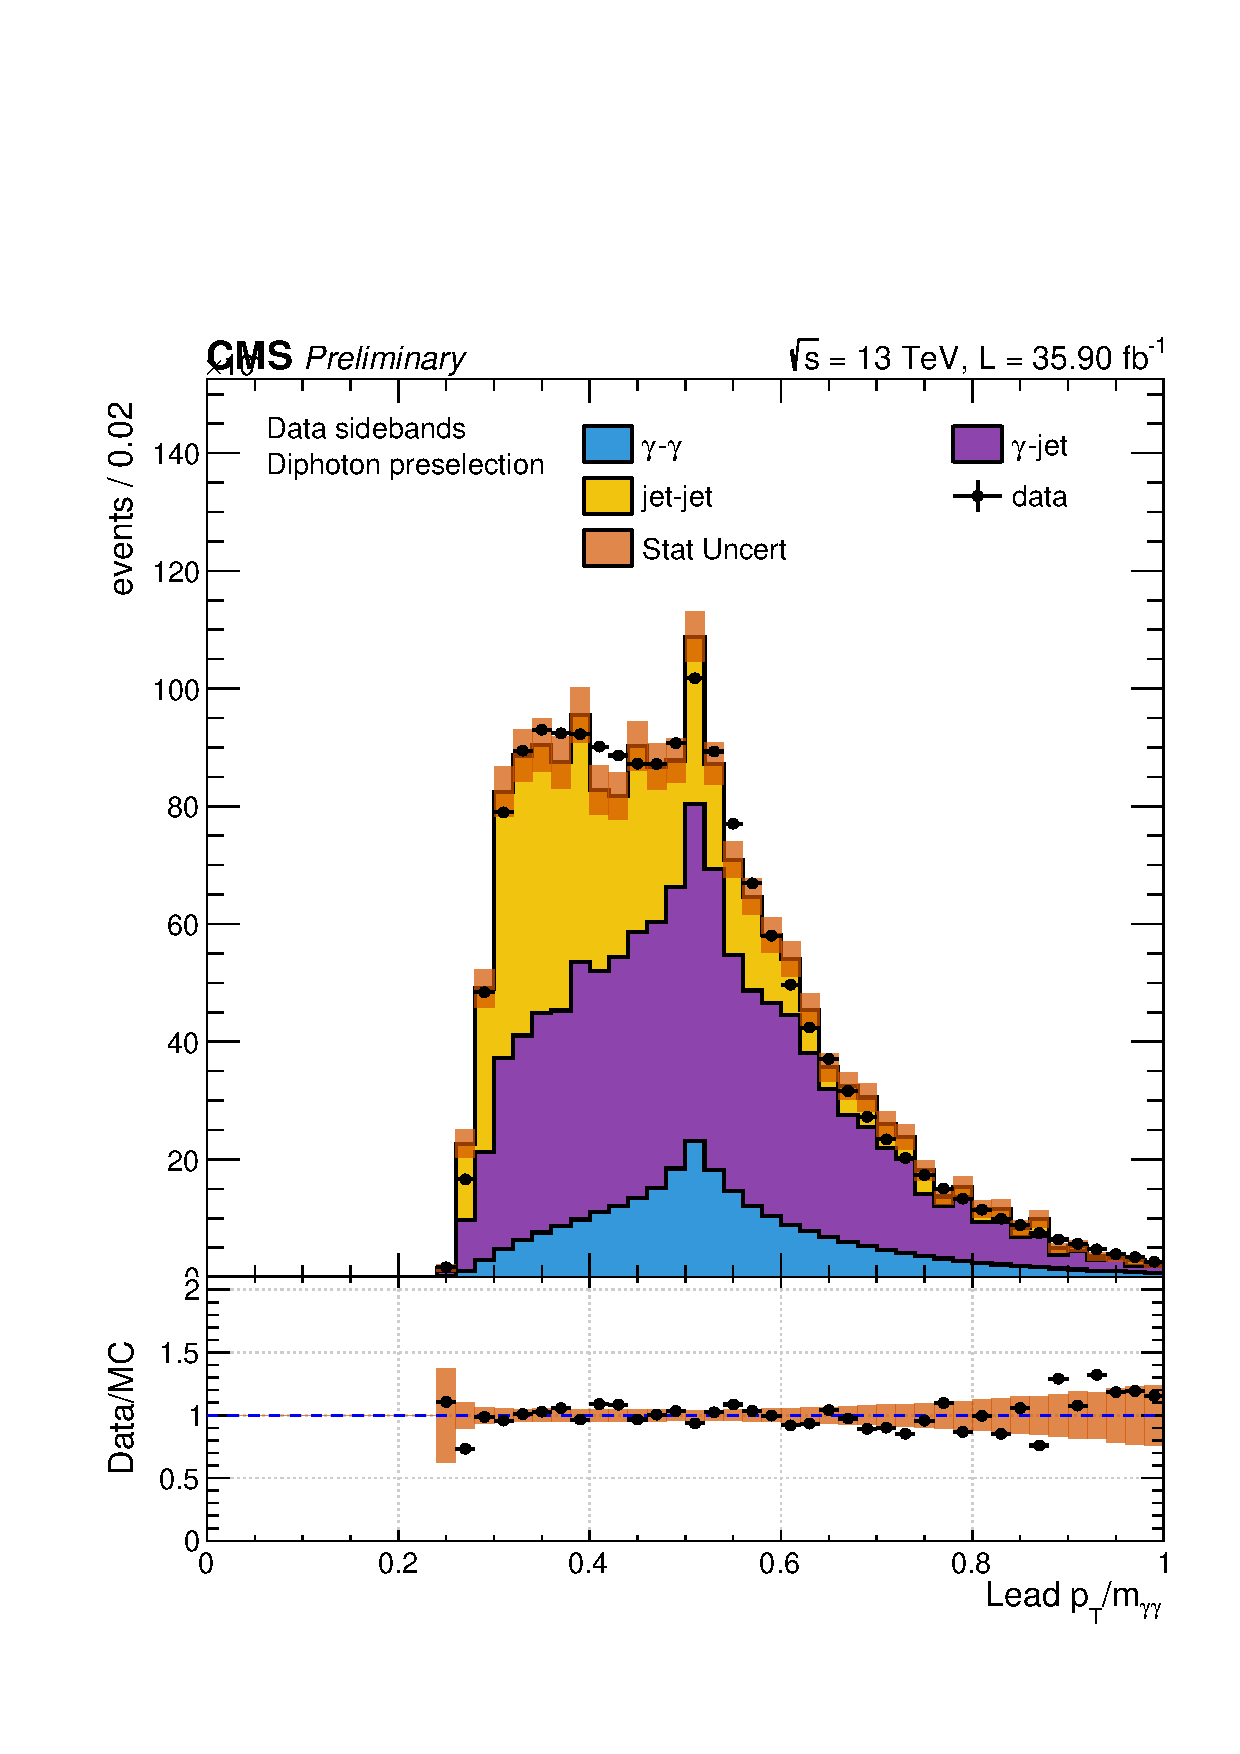
\includegraphics[width=0.49\textwidth]{Figures/Categorisation/leadptom_2016.pdf}
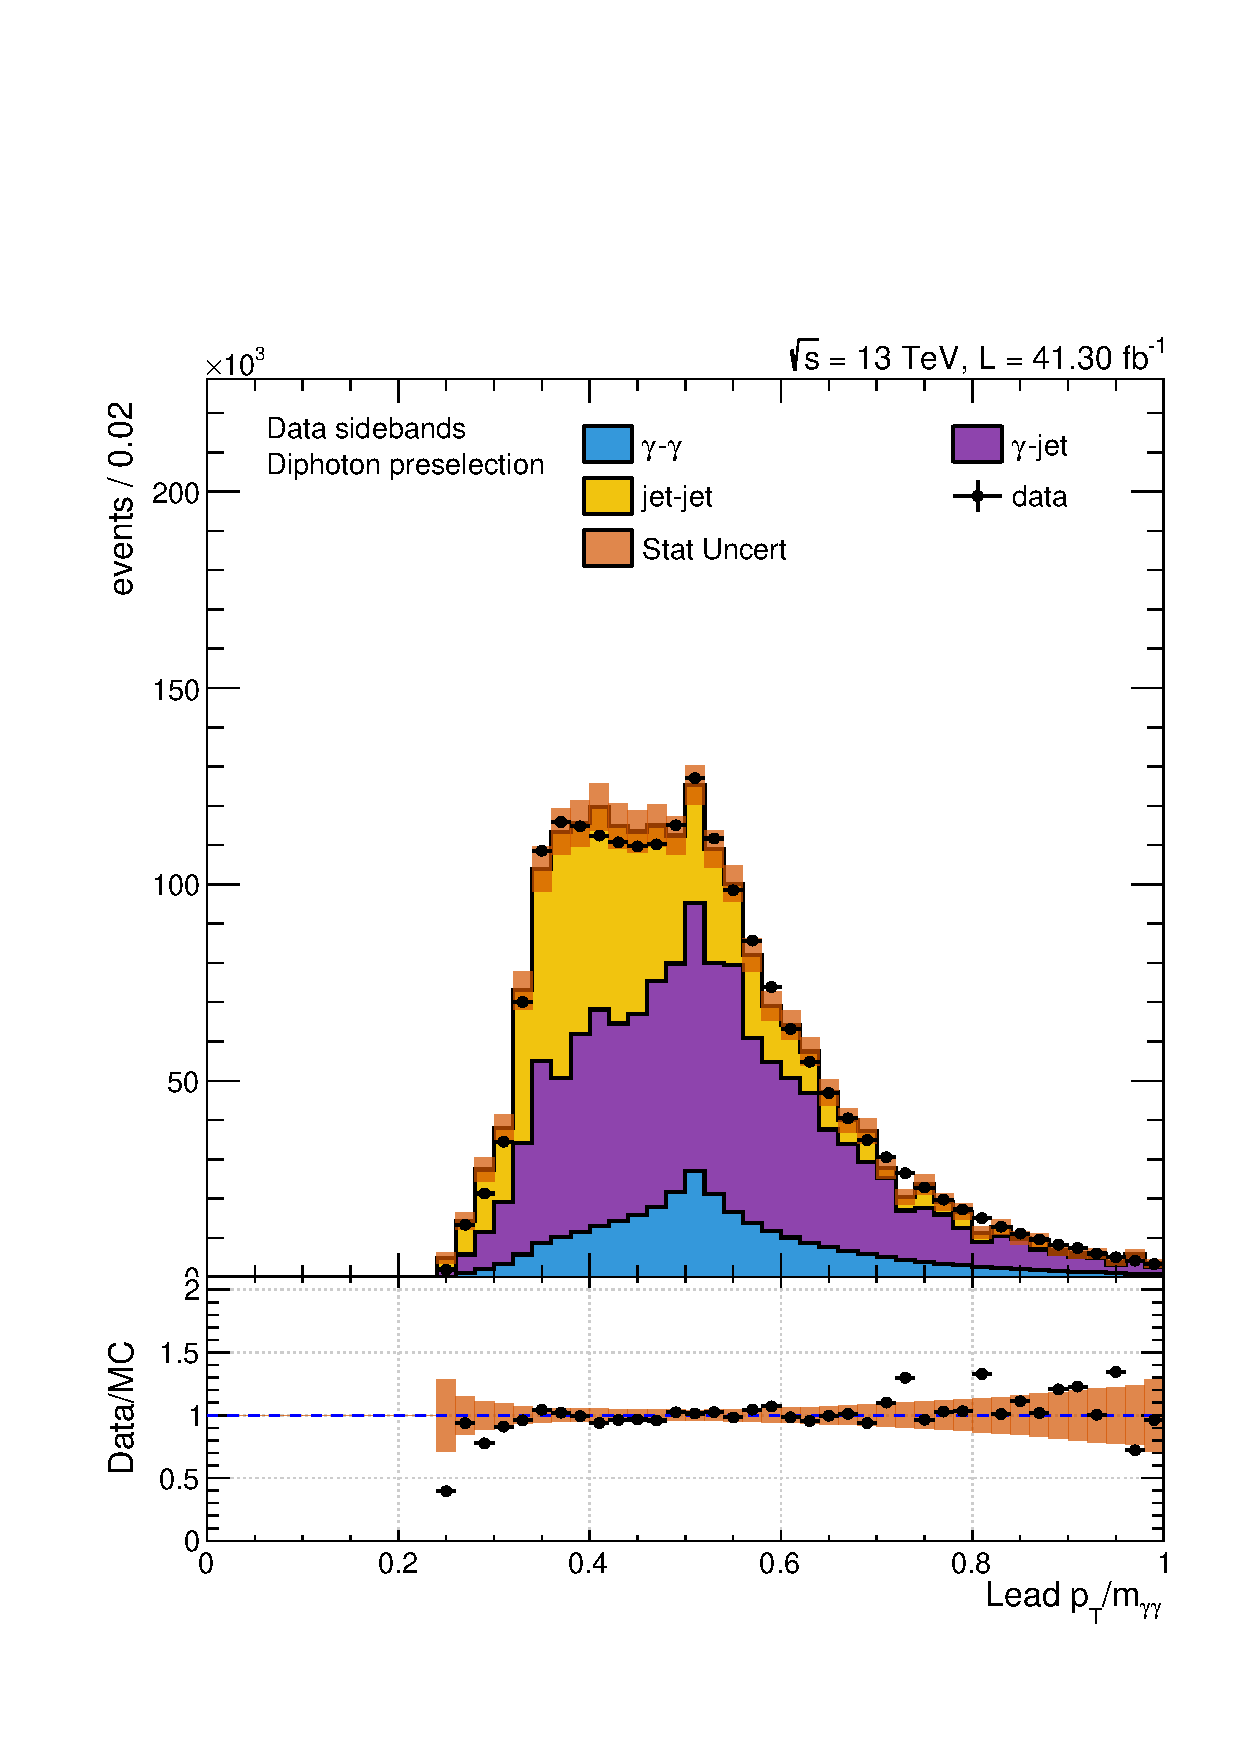
\includegraphics[width=0.49\textwidth]{Figures/Categorisation/leadptom_2017.pdf}
\caption{
  Distribution of the lead photon $\pt/\mgg$ in background (stacked histogram) 
  and data (black points) events.
  The statistical uncertainty is shown by the orange band.
  The left plot shows 2016 data and MC,
  with 2017 data and MC on the right.
}
\label{fig:cat_ptominput}
\end{figure}

None of the input variables above encode the preference for events with good mass resolution.
For this purpose, an additional weight is applied to signal events which increases the relative 
importance of events with better values of the diphoton mass resolution. 
The weight applied, $w_{res}$, is given by the formula

\begin{equation}
  w_{res} = \frac{p_{vtx}}{\srv} + \frac{1-p_{vtx}}{\swv}
\end{equation}

This ensures that the classifier output score is higher for events 
which have a relatively low expected diphoton mass resolution.
Finally, the signal and background samples are divided into a training and a test set,
containing 70\% and 30\% of the total number of events respectively.
With this configuration of input variables, signal and background events, and event weights, 
the classifier is trained and its performance evaluated using the XGBoost software package~\cite{XGBoost}.

The performance of the training is evaluated using a receiver operating characteristic (ROC) curve, 
where the signal efficiency is plotted as a function of the background efficiency,
with each point corresponding to a specific threshold value placed on the classifier output score.
The area under the ROC curve is used to gauge the performance of a given classifier; 
a higher area corresponds to more effective discrimination between signal and background.
For the 2016 and 2017 trainings, the areas under the respective ROC curves are 0.77 and 0.78.
%TODO update these numbers

This metric is utilised to compare the performance of the classifier training 
with different values of the BDT's so-called hyper-parameters.
These hyper-parameters are arbitrary parameters of the BDT, 
which are not learned but instead affect how the learning algorithm behaves.
The most important hyper-parameters affect the extent to which 
the algorithm learns the specific detail of the training sample provided.
If a classifier has learnt features from the training set inputs
which are due solely to statistical fluctuations and not a more general feature of the signal, 
over-training can result.
To check for potential over-training, the training score as measured by area under the ROC curve 
of the training set is compared with the score from the independent test set.
If the test set score is significantly higher than that of the training set, 
the classifier has been over-trained.
The default classifier hyper-parameters display no overtraining.
A coarse hyper-parameter optimisation procedure is then performed, 
in which each hyper-parameter is varied individually.
No significant improvement without overtraining is found, 
and therefore the default training parameters are used.

An additional parameter which can be optimised is the relative weight 
of the signal and background samples.
With the default sample weights corresponding to the SM sample cross section, 
the two classes are highly imbalanced.
This imbalance can cause suboptimal learning in the classifier.
To check this, the classifier is trained in a scenario 
where the signal event weights are increased by a uniform factor, 
such that the total sum of weights for signal and background is equal.
This is purely as a technical change to the training 
designed to improve the learning outcomes of the classifier.
When evaluating the performance, the default event weights are used.
Equalising the total weights in this way results in a modest improvement in performance.
The areas under the ROC curves become 0.80 and 0.82 for the 2016 and 2017 datasets respectively.
%TODO update these numbers
The improvement is relatively small, 
but is however larger than the variation 
in training performance induced by either changing the random seed used for training or 
choosing different subsets of the input data for training and testing.
Therefore we choose to use this training scenario for the final classification.
The hyper-parameter optimisation procedure was repeated 
and no significant improvement was obtained.

The ROC curves for the two different event weighting scenarios are shown in Figure~\ref{fig:cat_ROCs}.
It is evident that the scenario with equalised weights has slightly superior performance.
In addition, the relative importance of each feature is shown in Figure~\ref{fig:cat_importance}.
This plot serves as validation that the classifier is learning 
sensible features of the input dataset.
%TODO add ROC curve and feature importance plots here.

Validation of the diphoton BDT is performed using \Zee events, 
where simulated Drell-Yan events are compared with data.
This validation is important because although the background model used in the analysis 
is entirely data-driven, the signal model is taken from simulation.
Therefore it is necessary to ensure that there is reasonable agreement 
between data and simulation for signal-like objects,
for both the inputs to the diphoton BDT and the output score itself.
In this \Zee control region, the electrons are reconstructed as photons, 
and the presence of an electron pair with invariant mass $80 < m_{ee} < \SI{100}{GeV}$ is required.
Otherwise the event selection is the same as the analysis selection for diphoton events, 
except for the additional requirement that the leading electron $\pt > \SI{40}{GeV}$.
This requirement is necessary to ensure that no bias is introduced by the electron trigger, 
which has selection thresholds at $\pt = \SI{32}{GeV}~(\SI{35}{GeV})$ for 2016 (2017) data.

Figure~\ref{fig:cat_diphoBDT} shows the output score of the diphoton BDT for data and simulation.
The effect of two systematic uncertainties which affect the diphoton BDT are included;
these are the shift in the photon identification BDT score, 
and the uncertainty on the photon energy resolution.
Good agreement is observed between the data and simulation in both years, 
with all discrepancies covered by the statistical and systematic uncertainties.

\begin{figure}[hptb]
\centering
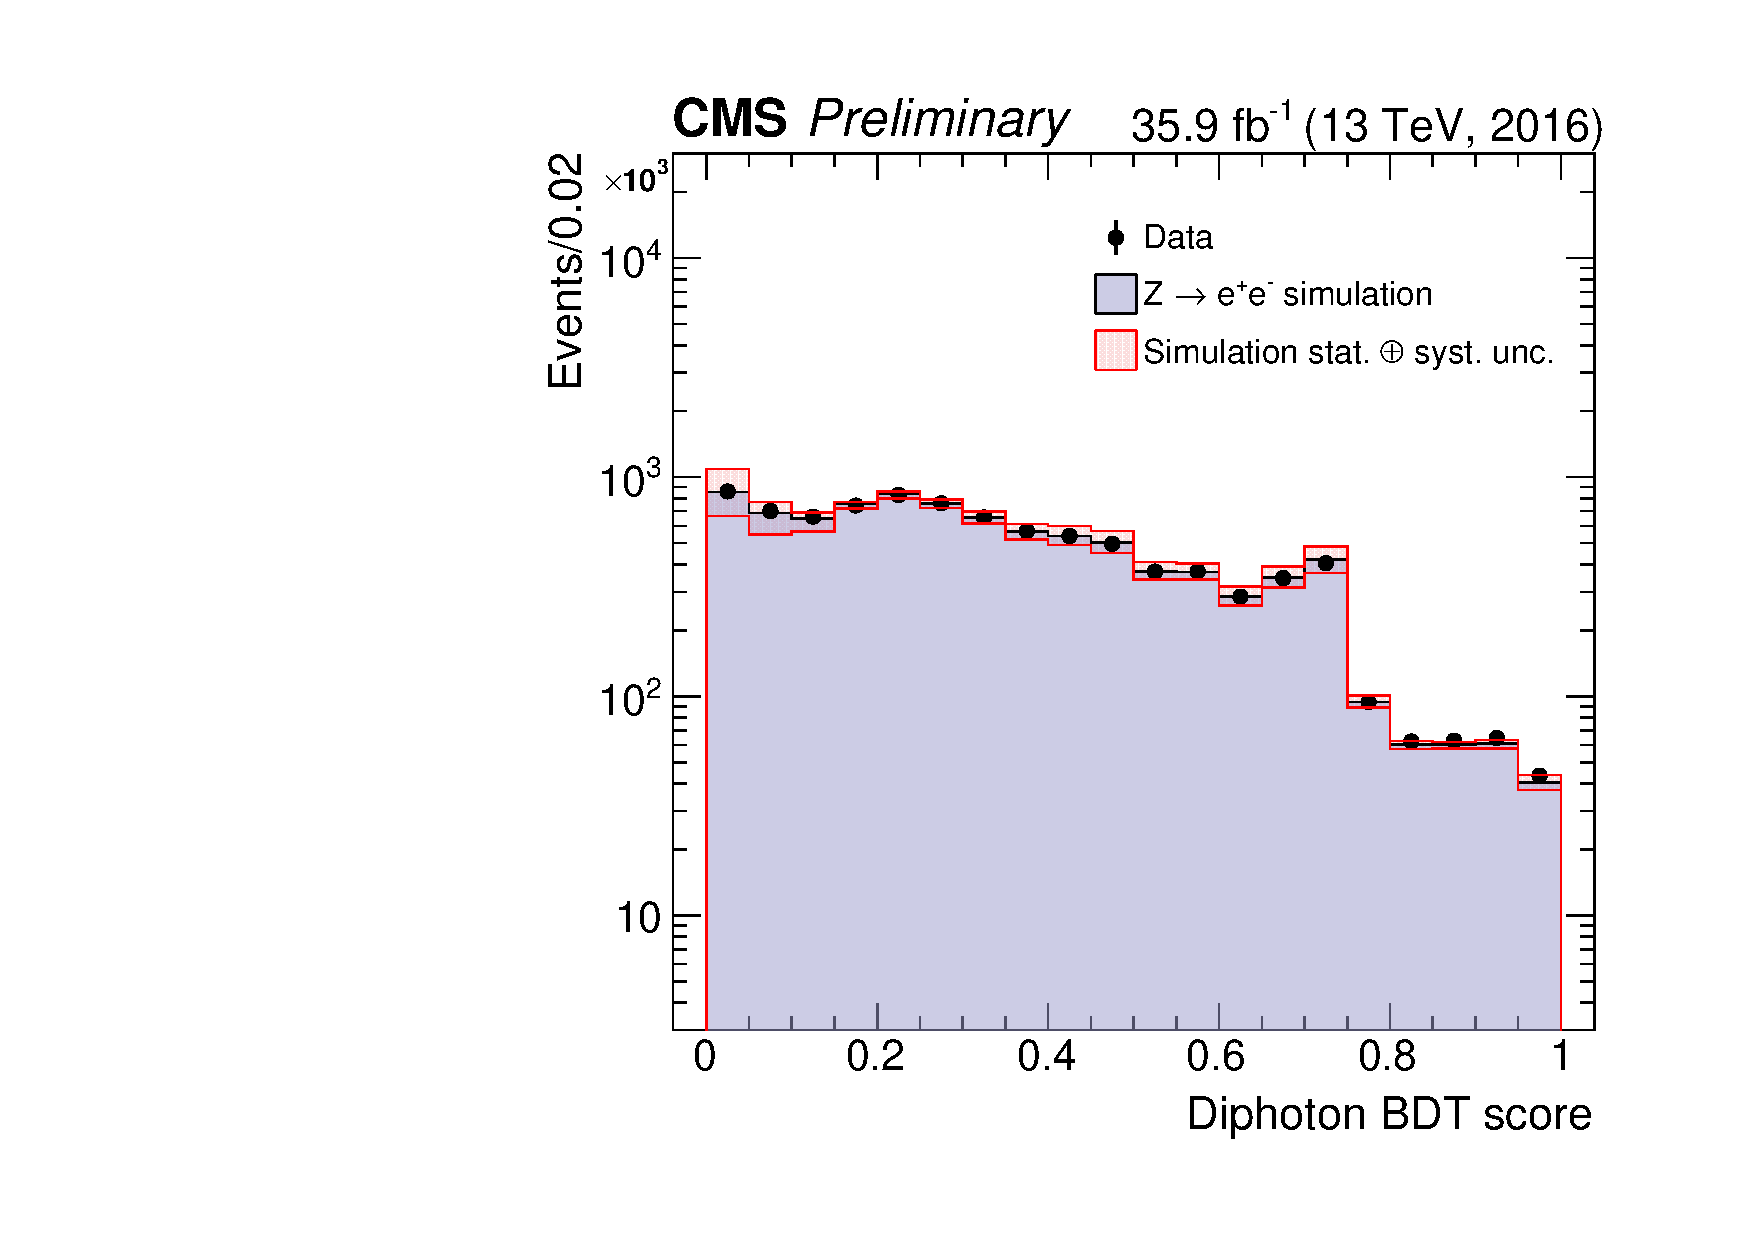
\includegraphics[width=0.7\textwidth]{Figures/Categorisation/DiphoBDT_2016.pdf}
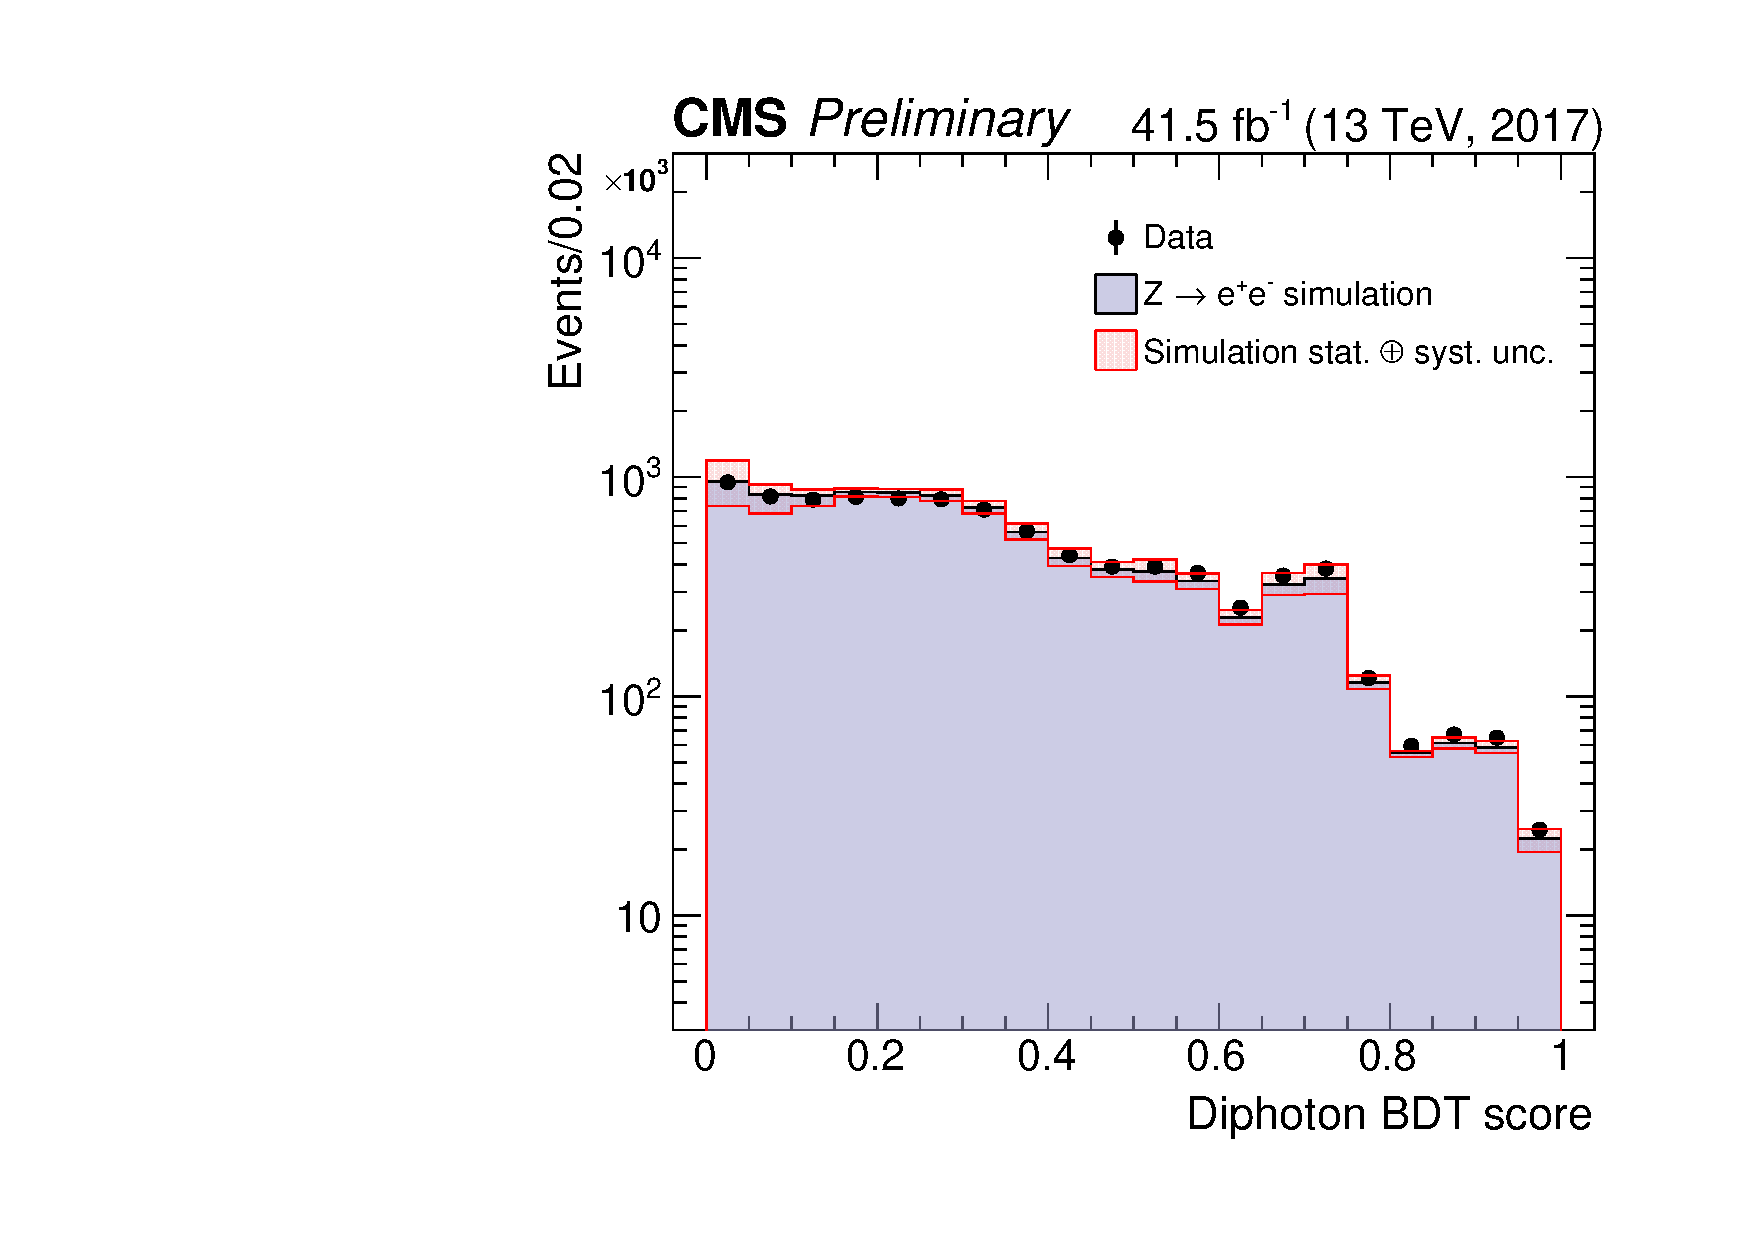
\includegraphics[width=0.7\textwidth]{Figures/Categorisation/DiphoBDT_2017.pdf}
\caption{
  Score of the diphoton BDT in $\Zee$
  events where the electrons are reconstructed as photons.
  The points show the score for data, the histogram shows
  the score for simulated Drell--Yan events, including statistical and 
  systematic uncertainties (pink band).
  The top plot shows 2016 data and MC,
  with 2017 data and MC on the bottom.
}
\label{fig:cat_diphoBDT}
\end{figure}

\subsection{Category definitions}

Once the diphoton BDT has been constructed, 
a category optimisation procedure can be performed for each Stage 1 bin independently.
The reconstructed number of jets and \ptgg defines the category type into which a a given event falls.
Then, independently for each category type, 
an optimisation procedure is performed to define diphoton BDT boundaries 
for a given number of subcategories.
The Approximate Mean Significance (AMS) is used to define the figure of merit for the optimisation.
The value of the AMS metric corresponds to the expected significance of a signal 
from the likelihood ratio statistic for a simple counting experiment, 
neglecting the impact of systematic uncertainties.
Its derivation is outlined in Ref~\cite{Asymptotic}.
The aim of this analysis is not to maximise the significance of each stage 1 bin.
Maximising the AMS is instead a proxy for minimising the expected uncertainty for a given bin.
The formula for the AMS is given by 

\begin{equation*}
  AMS = \sqrt{ 2 \left( (S+B) \ln{\left(1+\frac{S}{B}\right)} - S \right) }
\end{equation*}

where $S$ is 68\% (corresponding to $\pm 1\sigma_{eff}$) of the number of signal events 
from the desired truth bin (not the total number of signal events), and $B$ is the background.
The value of B is calculated by performing an exponential fit to the background, 
and then integrating the number of events between $125 - \sigma_{eff} < \mH < 125 + \sigma_{eff}$.
This formula reduces to $S/\sqrt{S+B}$ in the limit of small $S/B$.
Results are found to be robust to the choice of metric; 
only in bins with a very low number of events (e.g. the BSM bins) 
does the AMS metric return different optimal diphoton BDT boundaries from the $S/\sqrt{S+B}$ metric, 
and then the differences are relatively small.

The optimisation procedure itself is performed using a random search. 
This is found to be more computationally efficient than a grid search.
After the diphoton BDT boundaries have been established, 
a cross-check is performed to ensure that a sensible minimum has been found.
This is done by scanning the diphoton BDT value individually for each category type and each boundary; 
if a slightly better performing point is found in the vicinity, 
it replaces the value returned by the random search.
In general, the results of the random search are found to be robust.

This optimisation process is repeated for different numbers of categories.
No improvement beyond two categories per target STXS bin is observed, 
except for the 0J bin, which requires three categories.
The boundaries chosen and the expected number of signal and background events, 
together with the expected significance, 
are shown in Table~\ref{tab:cat_ggHsignificance2016} and Table~\ref{tab:cat_ggHsignificance2017} 
for 2016 and 2017 simulation and data respectively.

\begin{table}
  \begin{centering}
    \begin{tabular}{ r | c | c | c | c } 
    \hline 
    Category         & Diphoton BDT cut & Signal & Background & Significance ($\sigma$) \\
    \hline 
    0J Tag 0         & 0.851            & 145    & 1000       & 4.48                    \\
    0J Tag 1         & 0.796            & 201    & 2973       & 3.64                    \\
    0J Tag 2         & 0.586            & 238    & 9263       & 2.46                    \\
    \hline           
    1J low  Tag 0    & 0.832            & 36     & 462        & 1.67                    \\
    1J low  Tag 1    & 0.718            & 45     & 1635       & 1.11                    \\
    1J med  Tag 0    & 0.866            & 17     & 1042       & 1.60                    \\
    1J med  Tag 1    & 0.749            & 39     & 7755       & 1.38                    \\
    1J high Tag 0    & 0.908            & 5.5    & 18         & 1.14                    \\
    1J high Tag 1    & 0.810            & 6.6    & 112        & 0.61                    \\
    1J BSM  Tag 0    & 0.917            & 3.0    & 7.4        & 0.89                    \\
    \hline           
    GE2J low  Tag 0  & 0.833            & 4.8    & 142        & 0.39                    \\
    GE2J low  Tag 1  & 0.709            & 6.7    & 571        & 0.28                    \\
    GE2J med  Tag 0  & 0.869            & 8.3    & 65         & 0.99                    \\
    GE2J med  Tag 1  & 0.757            & 17     & 462        & 0.80                    \\
    GE2J high Tag 0  & 0.910            & 9.1    & 33         & 1.45                    \\
    GE2J high Tag 1  & 0.811            & 10     & 158        & 0.81                    \\
    GE2J BSM  Tag 0  & 0.938            & 9.7    & 9.4        & 2.48                    \\
    GE2J BSM  Tag 1  & 0.865            & 4.9    & 27         & 0.86                    \\
    \hline 
    \end{tabular}
    \caption{The chosen diphoton BDT boundaries, 
    the expected number of signal and background events, 
    and the expected significance of each category in the ggH phase space 
    for 2016 data and simulation, assuming an integrated luminosity of \SI{35.9}{\fbinv}.}
    \label{tab:cat_ggHsignificance2016}
  \end{centering}
\end{table}

\begin{table}
  \begin{centering}
    \begin{tabular}{ r | c | c | c | c } 
    \hline 
    Category         & Diphoton BDT cut & Signal & Background & Significance ($\sigma$) \\
    \hline 
    0J Tag 0         & 0.840            & 217    & 2042       & 4.72                    \\
    0J Tag 1         & 0.769            & 250    & 5063       & 3.49                    \\
    0J Tag 2         & 0.615            & 201    & 9669       & 2.03                    \\
    \hline                                                                              
    1J low  Tag 0    & 0.817            & 41     & 676        & 1.58                    \\
    1J low  Tag 1    & 0.652            & 42     & 2466       & 0.84                    \\
    1J med  Tag 0    & 0.881            & 8.5    & 45         & 1.18                    \\
    1J med  Tag 1    & 0.760            & 43     & 872        & 1.46                    \\
    1J high Tag 0    & 0.910            & 5.5    & 20         & 1.10                    \\
    1J high Tag 1    & 0.824            & 7.6    & 109        & 0.71                    \\
    1J BSM  Tag 0    & 0.775            & 4.9    & 1.2        & 2.02                    \\
    \hline                                                                              
    GE2J low  Tag 0  & 0.861            & 1.9    & 44         & 0.27                    \\
    GE2J low  Tag 1  & 0.709            & 8.0    & 649        & 0.31                    \\
    GE2J med  Tag 0  & 0.835            & 11     & 177        & 0.87                    \\
    GE2J med  Tag 1  & 0.786            & 6.9    & 10         & 1.74                    \\
    GE2J high Tag 0  & 0.916            & 6.3    & 24         & 1.17                    \\
    GE2J high Tag 1  & 0.815            & 10     & 163        & 0.78                    \\
    GE2J BSM  Tag 0  & 0.901            & 11     & 23         & 2.15                    \\
    GE2J BSM  Tag 1  & 0.596            & 3.0    & 1.8        & 1.25                    \\
    \hline 
    \end{tabular}
    \caption{The chosen diphoton BDT boundaries, 
    the expected number of signal and background events, 
    and the expected significance of each category in the ggH phase space 
    for 2017 simulation and data, assuming an integrated luminosity of \SI{41.5}{\fbinv}.}
    \label{tab:cat_ggHsignificance2017}
  \end{centering}
\end{table}

\section{Vector boson fusion categorisation}
\subsection{Signal bin definitions}

The VBF process is divided into five particle level bins at stage 1 of the STXS framework.
Events where the Higgs boson is produced in association with a vector boson (VH, where V = W or Z) 
and the vector boson decays hadronically are included together with VBF.
In this region, there are two bins defined analogously to the VBF-like bins for ggH production, 
requiring a dijet with $m_{jj} > \SI{400}{GeV}$ and $\Delta\eta > 2.8$, 
split by a \SI{25}{GeV} boundary in \ptHjj.
In addition, there is a ``VH-like" bin, 
which requires the presence of a dijet with $60 < m_{jj} < \SI{120}{GeV}$. 
A ``BSM-like" bin is also defined, where the \pt of the leading jet is greater than \SI{200}{GeV}.
All remaining events fall into the ``VBF rest" bin.
Each bin is exclusive; all bins, except for the BSM bin, 
are required to have the leading jet $\pt < \SI{200}{GeV}$.
Table \ref{tab:cat_VBFfractions} shows a summary of the definition of each bin 
and the corresponding fraction of the total VBF cross section.
The inclusive VBF cross section is \SI{3.779}{pb} at $\mH = \SI{125.09}{GeV}$~\cite{YR4},
computed at approximately next-to-next-to-leading (NNLO) order in QCD and NLO in EW,
of which approximately \SI{3.52}{pb} is within $|y_H| < 2.5$.
For hadronic VH production, 
the cross section at $\mH = \SI{125.09}{GeV}$ of \SI{1.54}{pb}~\cite{YR4}
is computed at NNLO in QCD and NLO in EW, 
with around \SI{1.37}{pb} within $|y_H| < 2.5$.

\begin{table}
  \begin{centering}
    \begin{tabular}{ r | c | c | c | c } 
    \hline
    Region & Definition & VBF fraction & VH fraction & Cross section (pb) \\ 
    \hline
    BSM                      & Leading jet $\pt > 200 GeV$             &  4.6\%                  & 5.4\%                   & 0.23                  \\ 
    \hline
    \multirow{2}{*}{2J-like} & $\ge$ two jets, $|\Delta\eta| > 2.8$,     & \multirow{2}{*}{25.8\%} & \multirow{2}{*}{0.4\%}  & \multirow{2}{*}{0.91} \\
                             & $m_{jj} >$ 400 GeV, $\ptHjj <$ 25 GeV    &                         &                         &                       \\
    \hline
    \multirow{2}{*}{3J-like} & $\ge$ two jets, $|\Delta\eta| > 2.8$,     & \multirow{2}{*}{9.0\%} & \multirow{2}{*}{1.7\%}  & \multirow{2}{*}{0.34} \\ 
                             & $m_{jj} >$ 400 GeV, $\ptHjj >$ 25 GeV    &                         &                         &                       \\
    \hline
    VH-like                  & $\ge$ two jets, $60 < m_{jj} < 120 GeV$ &  2.3\%                  & 34.5\%                  & 0.55 \\
    \hline
    Rest                     & All other VBF events                     & 59.2\%                  & 57.9\%                  & 2.86 \\ 
    \hline
    \end{tabular}
    \caption{The particle level definition of each VBF stage 1 bin 
    and the corresponding fractional and absolute cross sections.
    The fractions reported are normalised relative to inclusive VBF or VH hadronic production, 
    whilst the cross sections are the sum of the VBF and VH hadronic values.
    The fractions are estimated from simulated VBF and hadronic VH \Hgg events 
    within the region $|y_H| < 2.5$.
    Details of the simulated samples can be found in Section~\ref{chap:objects}.
    Each bin is exclusive; all bins except the BSM bin 
    are required to have the leading jet $\pt < 200$ GeV.
    }
    \label{tab:cat_VBFfractions}
  \end{centering}
\end{table}

Different categorisation scenarios are considered for the VBF process.
Ideally categories would be constructed to target each stage 1 bin.
However, the experimental sensitivity to the BSM-like, VH-like, and VBF rest bins is limited.
Care is therefore taken not reduce the sensitivity to inclusive VBF production when designing 
the categories for each of these categories.

The bins which can be most precisely measured are the 2J-like and 3J-like VBF bins.
In addition to migrations between the categories targeting each bin, 
there is substantial contamination from events with two jets arising from ggH production.
For this reason the dijet BDT is trained to discriminate between ggH and VBF events.
The categorisation is then performed using the detector level versions 
of the quantities used to define the bins: \mjj, \ptHjj, and leading jet \pt, 
before the dijet and diphoton BDTs are used 
to reduce the respective number of ggH and background events entering the categories.

\subsection{Dijet BDT}

The dijet BDT is trained to discriminate VBF events from both background and ggH events.
This is made possible due to the distinctive signature of VBF events, 
which typically have two jets with large separation in pseudorapidity and high invariant mass.
Therefore the input variables to the dijet BDT consist of primarily of jet-related variables.
In addition, the jets in VBF events originate from quarks, 
whereas ggH events typically originate from gluons.
This results in subtle differences in the internal structure of the jet objects, 
as discussed in Chapter~\ref{chap:HGCAL}.
The variables used there do not significantly improve the dijet BDT performance;
however it has been shown that more sophisticated techniques using neural network classifiers
and detailed jet image inputs can improve the performance~\cite{JackThesis}.
The full set of input variables for the dijet BDT are:
\begin{itemize}
\item the transverse momentum of the two leading photons, divided by the diphoton mass, $\pt^{1,2}/\mgg$;
\item the transverse momentum of the two leading jets, $\pt^{j1,j2}$;
\item the invariant mass of the dijet, \mjj;
\item the magnitude of the difference in pseudorapidity of the two leading jets, $|\Delta\eta|$;
\item the magnitude of the difference in azimuthal angle 
      between the two leading jets, $|\Delta\phi_{jj}|$;
\item the magnitude of the difference in azimuthal angle 
      between the diphoton and dijet, $|\Delta\phi_{\gamma\gamma,jj}|$;
\item the minimum angular separation between either of the two leading photons 
      and either of the two leading jets, $\Delta R_{\textrm{min}}(\gamma,j)$;
\item the centrality variable, which is given by:
\begin{equation}
C_{\gamma\gamma} = \mathrm{exp}\left(-\frac{4}{(\eta_{j1} - \eta_{j2})^{2}}\left( \eta_{\gamma\gamma} - \frac{\eta_{j1} + \eta_{j2}}{2} \right)^{2}\right)
\end{equation}
where $\eta_{j1}$ and $\eta_{j2}$ are the pseudorapidities of the 
leading and subleading jets respectively.
\end{itemize}

%TODO describe what was done in the past with the fully MC inputs here
%including discussion of the issues and why they result in suboptimal results
%don't forget the different preselections, and full definition of what we use now

In previous versions of the analysis \cite{HIG-16-040}, 
both the signal and background for the dijet BDT training have been taken directly from simulation. 
However there are a limited number of events in the prompt-fake and fake-fake backgrounds
which pass the analysis preselection, 
and this problem is exacerbated by applying additional requirements on the dijet system.
%Have a go at explaining why here?
Consequently, there are few events with which to train the dijet BDT, 
and those events which are present have an extremely high cross-section.
This results in multiple issues that reduce the effectiveness of the dijet BDT.
If these high-weight events are included in the training, 
the classifier assigns too much importance to specific instances 
and does not succesfully learn generalised features of the input datasets.
Attempts have been made to mitigate this, 
the first of which is to reduce the weight of the QCD events by a factor of 25.
In addition, the VBF preselection is loosened in 
order to include more events in the training.
The standard VBF preselection consists of the analysis preselection 
with the additional requirements of $\pt > 40 (30)$ GeV for the leading (subleading) jet, 
$\mjj > \SI{250}{GeV}$ and photon identification BDT score of greater than -0.2 for both photons.
The loosened version reduces the \pt thresholds by \SI{10}{GeV} each, 
the \mjj threshold to \SI{100}{GeV}, and removes the tighter photon identification requirement.
This slightly improves the training performance; 
however the background rejection is still suboptimal 
due to the change in phase space and reduction in event weights.
Furthermore, this makes the simulation very difficult to validate against data
since the distributions are highly discontinuous.
An illustration of the effect is shown in Figure~\ref{fig:cat_lowstats}, 
which shows the output of the dijet BDT in the previous analysis~\cite{HIG-16-040}.

An alternative solution to this problem is to use events from a data control region 
to replace the MC samples with low numbers of events.
This method is used for the first time in this analysis;
the outline of the procedure is as follows:
\begin{itemize}
\item Define a control region by inverting the photon identification BDT requirement 
      for events entering the VBF signal region;
\item Use simulation to compute the relative fraction of events in the signal region and control region, 
      for each photon, as a function of the photon kinematics;
\item Apply these factors as event weights to the data in the control region 
      and use these events to replace the simulation of prompt-fake and fake-fake events in the training.
\end{itemize}
The details of this procedure are described below.

%TODO go on to describe the data-driven replacement method here
%including full details of how it works, its validation and improvement it brings

\subsection{Category definitions}

%TODO here discuss the previous approach with the combined BDT, its inputs, rationale etc
%then go on to describe the different scenarios considered, and their (dis)advantages
%once the optimal scheme is identified, give the final tag definitions

In previous versions of the analysis, 
the categories targeting VBF were defined using the so-called ``combined BDT".
The combined BDT is designed to incorporate both the dijet and diphoton information 
in order to optimally construct the VBF categories.
Its input variables are:
\begin{itemize}
\item the diphoton BDT score
\item the dijet BDT score
\item the transverse momentum of the two leading photons, divided by the diphoton mass, $\pt^{1,2}/\mgg$;
\end{itemize}
The combined BDT is trained with VBF against the three sources of SM background, 
using simulated events in each case.
Gluon fusion is not included in the training because it is found to worsen the performance 
of the combined BDT to reject true background.
Since these backgrounds have a greater impact on the final sensitivity 
than the contamination from other signal processes, 
this is considered a higher priority.
However it does mean that the ggH rejection of the combined BDT can be sub-optimal.
Here the efficacy of the combined BDT is combined with the more direct approach of 
defining the VBF categories by imposing thresholds on the diphoton and dijet BDT scores directly.

In addition, different possible categorisation scenarios are considered.
In Ref~\cite{HIG-16-040}, three inclusive categories are defined using the combined BDT.
For this analysis, further splitting using kinematic variables is required 
if the different VBF stage 1 bins are to be measured individually.
%However it is found that optimising for each stage 1 bin independently, 
%considering only one stage 1 bin as signal in each case, 
%reduces the overall sensitivity to the VBF process.
%Therefore when comparing different categorisation scenarios,
When comparing different categorisation scenarios,
the figure of merit considered is the total VBF significance, 
computed using the AMS metric with all VBF bins considered as signal.
Scenarios with additional splits following the stage 1 bin definitions 
will then be considered preferable, 
provided they do not substantially reduce the overall VBF significance.
The list of scenarios considered is as follows:
\begin{itemize}
\item list scenarios here
\end{itemize}

A random optimisation procedure is followed for each scenario considered, 
using the same methodology as for the ggH categories.
In the case of the approach applying only thresholds on the diphoton and dijet BDT output scores, 
the values of the thresholds on the two BDTs are optimised simultaneously for each category.
The resulting significance values of each scenario for the 2016 and 2017 datasetsis 
are shown in Tables~\ref{tab:cat_VBFscenarios2016} and \ref{tab:cat_VBFscenarios2017} respectively.
The performance of the combined BDT approach is compared with the approach using the diphoton 
and dijet BDT scores directly in each case.
The results demonstrate that there is no substantial reduction in the overall VBF significance
when the most granular categorisation scenario is optimised in this way;
it is therefore considered the best scenario for facilitating measurements of individual stage 1 bins.

Tables~\ref{tab:cat_VBFcuts2016} and \ref{tab:cat_VBFcuts2016} show the final thresholds 
for the diphoton and dijet BDTs in each category, 
together with the expected number of signal and background events and the per-category significance.
